\documentclass[tikz,border=8pt]{standalone}
\usepackage{tikz}
\usetikzlibrary{shapes,arrows,positioning}
\tikzstyle{proc}=[rectangle,draw,rounded corners,fill=blue!10,align=center,minimum width=3.4cm,minimum height=0.9cm,font=\small]
\tikzstyle{dec}=[diamond,draw,fill=green!10,align=center,aspect=2,font=\small]
\tikzstyle{term}=[rectangle,draw,rounded corners=8pt,fill=gray!15,align=center,minimum width=2.6cm,minimum height=0.9cm,font=\small\bfseries]
\tikzstyle{arr}=[->,thick]
\begin{document}
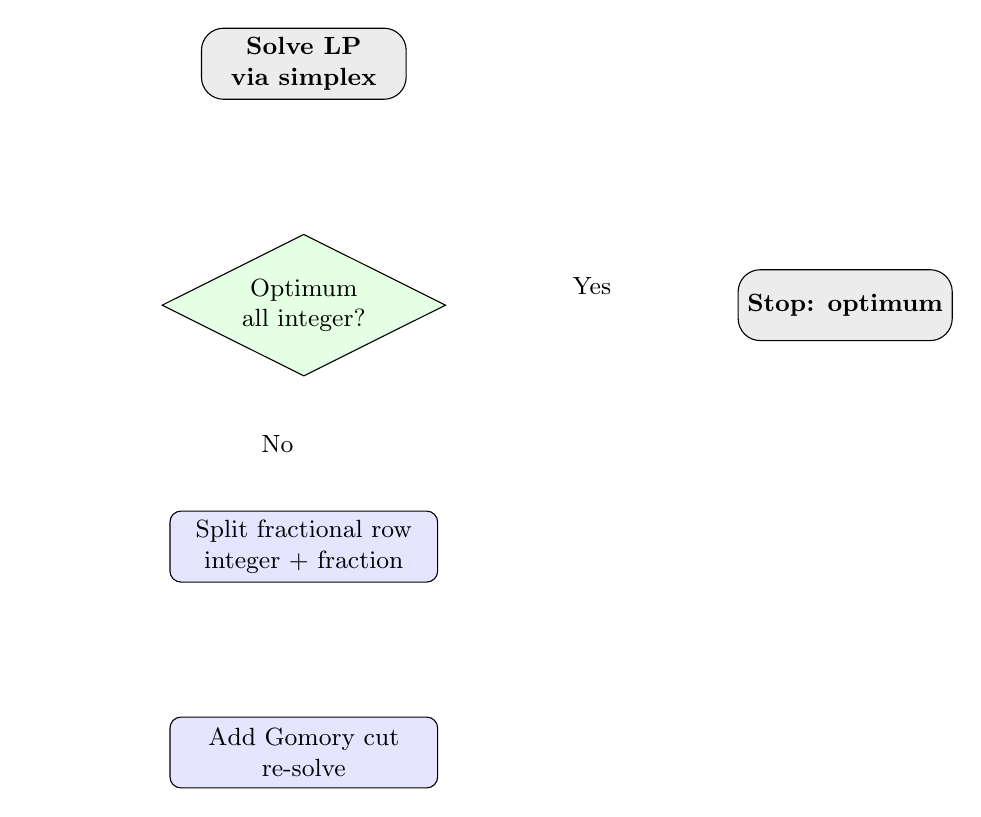
\begin{tikzpicture}[node distance=1.7cm]
\node[term] (A) {Solve LP\\via simplex};
\node[dec, below=of A] (B) {Optimum\\all integer?};
\node[term, right=of B, xshift=2.0cm] (C) {Stop: optimum};
\node[proc, below=of B] (D) {Split fractional row\\integer + fraction};
\node[proc, below=of D] (E) {Add Gomory cut\\re-solve};
\path[arr] (A) -- (B);
\path[arr] (B) -- node[above, font=\small] {Yes} (C);
\path[arr] (B) -- node[left, font=\small] {No} (D);
\path[arr] (D) -- (E);
\path[arr] (E.west) -- ++(-1.8cm,0) |- (B.west);
\end{tikzpicture}
\end{document}
